\documentclass{article}
\usepackage{amsmath}
\usepackage{titlesec}
\usepackage{graphicx}
\usepackage[margin=1in]{geometry}
\usepackage{hyperref}

% Title, date, and author
\title{Lab 1}
\author{Your Name, Collaborator's Name}
\date{\today}

\titleformat{\section}
  {\normalfont\normalsize\bfseries} % Format: font style, size, and weight
  {\thesection}{1em} % Label format and spacing
  {}
  \renewcommand{\thesubsection}{\thesection.\alph{subsection}}

\titleformat{\subsection}
  {\normalfont\small\bfseries} % Format: font style, size, and weight
  {\thesubsection}{1em} % Label format and spacing
  {}
\titleformat{\subsubsection}
  {\normalfont\small\bfseries} % Format: font style, size, and weight
  {\thesubsubsection}{1em} % Label format and spacing
  {}

\begin{document}
\begin{titlepage}
    \centering
    \vspace*{1in}
    
    {\Huge\bfseries Lab 1\par}
    \vspace{1.5cm}
    {\Large \today\par}
    \vspace{1.5cm}
    {\Large\itshape Antonio Pampalone 23586519 \\ Giuseppe Pisante 23610012\\ Martina Raffaelli 23616907 \par}
    
    \vfill
    
\includegraphics[width=0.3\textwidth]{FAU-Logo.png}\par\vspace{1cm} % Adjust the width as needed
   
\end{titlepage}

\newpage
\small

\section{Task 1.0}

\section{Task 1.1}

\section{Task 1.2}

\section{Task 1.3}

\section{Task 1.4}

Yes, there are noticeable differences in the contour plots when changing the spatial resolution and/or the time step.
Using a fixed spatial resolution of \( \Delta x = \Delta y = \frac{1}{40} \) with a number of time steps of 160, we observe that 
the solution becomes unstable because the time step violates the Von Neumann stability criterion for the explicit Euler method.

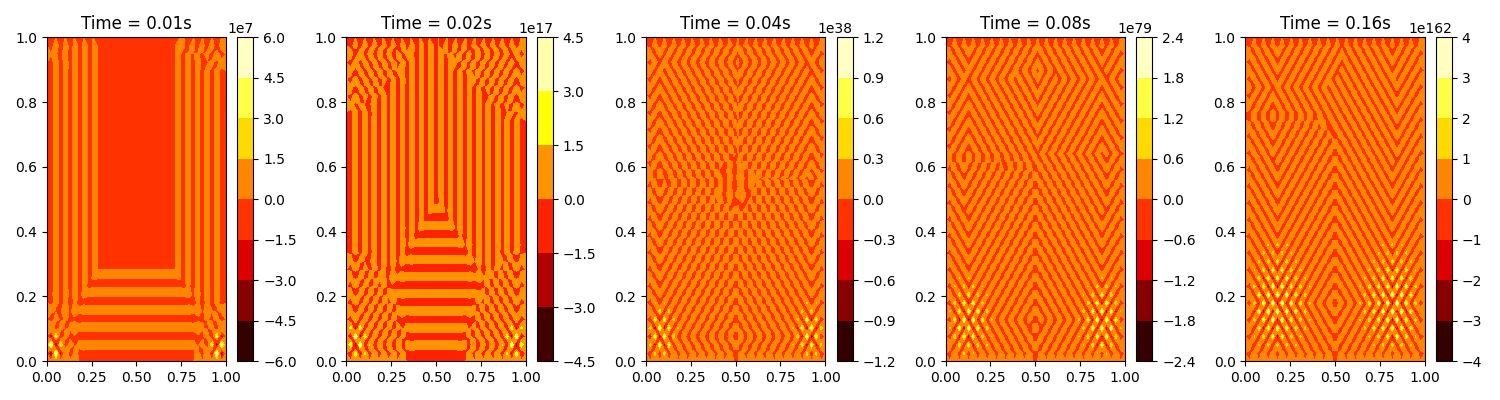
\includegraphics[width=\textwidth]{Figure_1.png}\par\vspace{1cm}

The stability condition ensures that errors introduced at each time step do not grow exponentially as
the computation progresses. In particular, for a 2D heat diffusion problem, this condition can be expressed as:

\[
\Delta t \leq \frac{\Delta x^2}{4}
\]

which implies that the minimum required number of time steps must be at least 1024. 
Infact, using a number of time steps of 1600 the solution becomes stable:

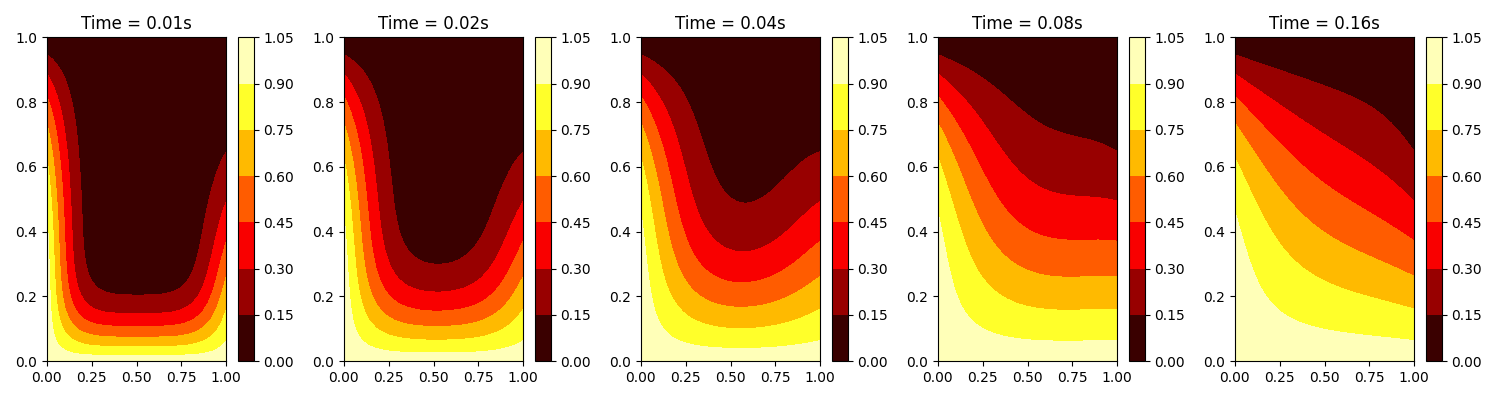
\includegraphics[width=\textwidth]{Figure_2.png}\par\vspace{1cm}

Similarly, using a finer spatial resolution of \( \Delta x = \Delta y = \frac{1}{100} \) with a number of
time steps of 1600 the solution becomes unstable because the minimum number of time steps for stability must be 6400.

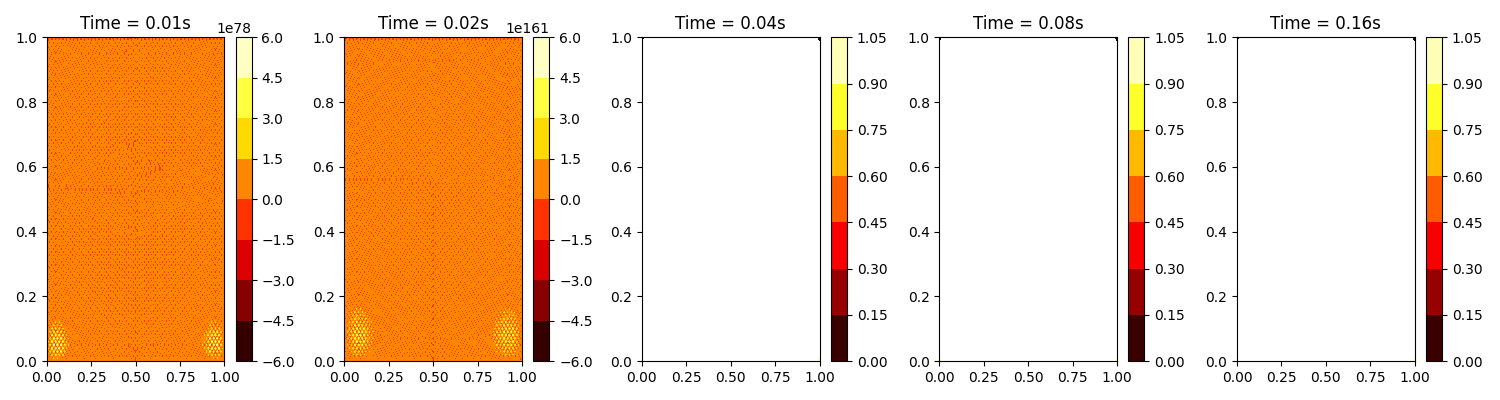
\includegraphics[width=\textwidth]{Figure_3.png}\par\vspace{1cm}

Higher spatial resolution allows for a more accurate representation of temperature but requires smaller
time steps to maintain stability. Infact, with a number of time steps of 6400, the solution becomes stable:

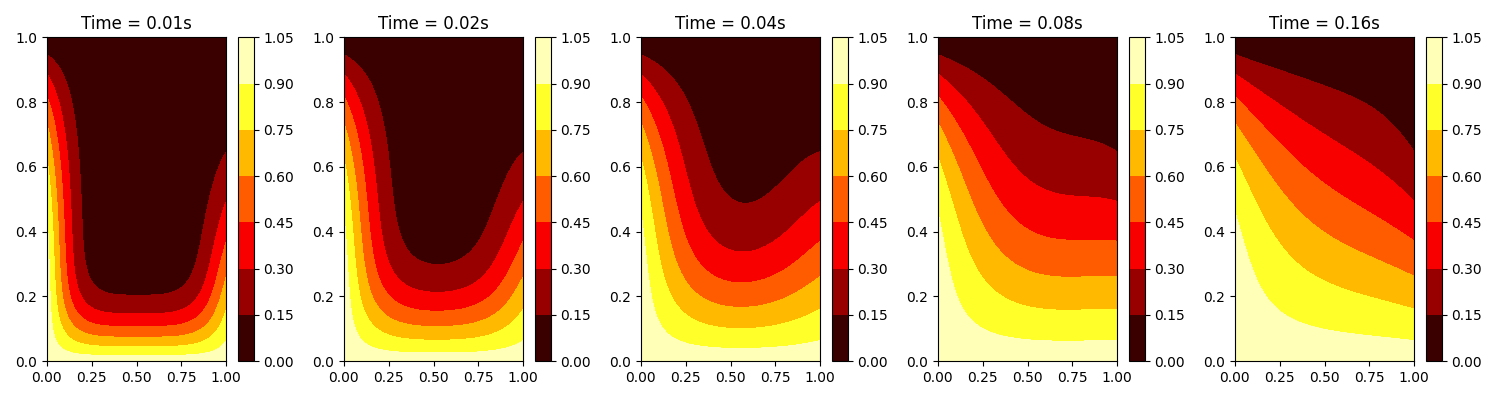
\includegraphics[width=\textwidth]{Figure_4.png}\par\vspace{1cm}

The stability of the solution depends on the ratio between \( \Delta t \) and \( \Delta x \). For finer grids, a smaller \( \Delta t \) 
is required to avoid instability. The choice of time values that are factors of 2 apart \( (t = 0.01, 0.02, 0.04, 0.08, 0.16) \) helps us
understand how heat diffusion evolves over time, allowing us to observe the progression of the temperature field at exponentially increasing 
intervals. Using exponentially increasing time steps provides a clear and efficient view of both the rapid initial diffusion and the slower, 
later stages, without requiring an excessive number of snapshots.


\begin{thebibliography}{9}
    \bibitem{GitHubRepo}
    \textit{CFD Repository},\\
    Available at: \url{https://github.com/GiuseppePisante/CFD.git}
    
    \bibitem{GitHubCopilot}
    \textit{GitHub Copilot},\\
    GitHub. Available at: \url{https://github.com/features/copilot}
    \end{thebibliography}

\end{document}